% =====================================================================
%  Лекция 5. Критерий согласия Колмогорова. Критерий омега-квадрат
%  Дата: 2026-10-15
% =====================================================================
\section[Критерий согласия Колмогорова. Критерий омега-квадрат]%
  {Критерий согласия Колмогорова. Критерий~\texorpdfstring{$\omega^2$}{омега-квадрат}}
\label{lec:05}

\subsection{Статистика Колмогорова}
\label{lec05:statistic}

Пусть задана генеральная совокупность~$\xi$ с функцией распределения~$F_\xi$
и выборка $X_{[n]} = (X_1, \ldots, X_n)$ из неё. Как и в критерии Пирсона
(раздел~\ref{lec04:pearson-test}), проверяем простую гипотезу
\[
  H_0 \colon F_\xi = F_0, \qquad H_1 \colon F_\xi \ne F_0,
\]
где $F_0$~--- полностью известная функция распределения. Дополнительно предполагаем,
что \textbf{$F_0$ непрерывна на~$\R$}: без этого всё дальнейшее неверно.

Идея: эмпирическая функция распределения $F_n^*$ приближает истинную~$F_\xi$
(теорема Гливенко--Кантелли), поэтому естественно смотреть, насколько далеко
$F_n^*$ отходит от гипотетической~$F_0$.

\begin{definition}
  \emph{Статистикой Колмогорова} называется
  \[
    D_n(X_{[n]}) = \sup_{x \in \R} \abs{F_n^*(x) - F_0(x)}.
  \]
\end{definition}

Так как $F_n^*$ и $F_0$ принимают значения в~$[0, 1]$, то $0 \le D_n \le 1$.

\subsubsection{Поведение при \texorpdfstring{$H_0$}{H0} и \texorpdfstring{$H_1$}{H1}}

\begin{itemize}
  \item \emph{Если верна $H_0$,} то $F_\xi = F_0$, и по теореме Гливенко--Кантелли
        (теорема~\ref{lec02:glivenko})
        \[
          D_n(X_{[n]}) = \sup_{x \in \R} \abs{F_n^*(x) - F_\xi(x)} \toas 0.
        \]
        Здесь нужна именно \emph{равномерная} сходимость: из поточечной
        $F_n^*(x) \toas F_0(x)$ при каждом~$x$ сходимость супремума не следует.
  \item \emph{Если верна $H_1$,} то $F_n^*$ сходится к истинной $F_\xi \ne F_0$, и
        \[
          D_n(X_{[n]}) \toas \sup_{x \in \R} \abs{F_\xi(x) - F_0(x)} > 0
        \]
        (тоже следствие теоремы Гливенко--Кантелли).
\end{itemize}
Итак, при $H_0$ статистика мала, при $H_1$ остаётся отделённой от нуля. Большие
значения $D_n$ свидетельствуют против~$H_0$.

\begin{remark}
  <<$D_n > 0$>> само по себе ничего не говорит: ступенчатая $F_n^*$ не может совпасть
  с непрерывной~$F_0$, поэтому $D_n > 0$ всегда, и при $H_0$ тоже.
  Различие между $H_0$ и $H_1$~--- в пределе: ноль или положительное число.
\end{remark}

\subsection{Распределение \texorpdfstring{$D_n$}{Dn} не зависит от \texorpdfstring{$F_0$}{F0}}
\label{lec05:distribution-free}

Чтобы построить критерий, нужно знать распределение $D_n$ при~$H_0$. Оказывается,
оно одно и то же для всех непрерывных~$F_0$.

\begin{lemma}[{\cite[гл.~14, лемма~2.1]{bure}}]
  \label{lec05:lemma}
  Если гипотеза $H_0$ верна и $F_0$ непрерывна на~$\R$, то распределение статистики
  $D_n(X_{[n]})$ не зависит от закона распределения генеральной совокупности
  (а зависит только от~$n$).
\end{lemma}

\begin{proof}
  Докажем при дополнительном предположении: существует интервал $(a, b)$,
  $-\infty \le a < b \le +\infty$, на котором $F_0$ строго возрастает, причём
  $F_0(a) = 0$, $F_0(b) = 1$ (при $a = -\infty$ или $b = +\infty$ понимаем это как
  пределы). Так устроены, например, нормальное, показательное, равномерное распределения.

  Так как $\P\{\xi \le a\} = F_0(a) = 0$ и $\P\{\xi > b\} = 1 - F_0(b) = 0$, то
  $\xi \in (a, b)$ п.н.; то же для каждого~$X_i$. На $(a, b)$ функция $F_0$ непрерывна,
  строго возрастает и пробегает все значения из $(0, 1)$, поэтому у неё есть обратная
  $F_0^{-1} \colon (0, 1) \to (a, b)$.

  \emph{Шаг~1: $F_0(\xi) \sim U[0, 1]$.} Пусть $y \in (0, 1)$. Для $\xi \in (a, b)$
  в силу строгого возрастания $F_0(\xi) \le y \iff \xi \le F_0^{-1}(y)$, поэтому
  \[
    \P\{F_0(\xi) \le y\} = \P\{\xi \le F_0^{-1}(y)\} = F_0\bigl(F_0^{-1}(y)\bigr) = y.
  \]
  При $y \le 0$ эта вероятность равна~$0$, при $y \ge 1$~--- единице. Это функция
  распределения равномерного закона на $[0, 1]$.

  \emph{Шаг~2: замена $y = F_0(x)$.} Положим $Y_i = F_0(X_i)$. Величины
  $Y_1, \ldots, Y_n$ независимы (как функции от независимых~$X_i$) и по шагу~1
  распределены по $U[0, 1]$, то есть $Y_{[n]} = (Y_1, \ldots, Y_n)$~--- выборка
  из равномерного распределения на~$[0, 1]$. Пусть $G_n^*$~--- её эмпирическая функция
  распределения. Для $x \in (a, b)$ снова из строгого возрастания
  \begin{align*}
    F_n^*(x) &= \frac1n \sum_{i=1}^n \Ind{X_i \le x}
              = \frac1n \sum_{i=1}^n \Ind{F_0(X_i) \le F_0(x)} \\
             &= \frac1n \sum_{i=1}^n \Ind{Y_i \le y}
              = G_n^*(y), \qquad y = F_0(x).
  \end{align*}
  При $x \le a$ и $x \ge b$ разность $F_n^*(x) - F_0(x)$ равна нулю (п.н.). Когда $x$
  пробегает $(a, b)$, $y = F_0(x)$ пробегает $(0, 1)$, поэтому
  \[
    D_n(X_{[n]}) = \sup_{x \in \R} \abs{F_n^*(x) - F_0(x)}
                 = \sup_{y \in [0, 1]} \abs{G_n^*(y) - y}.
  \]

  \emph{Шаг~3.} Правая часть~--- функция только от равномерной выборки $Y_{[n]}$,
  и $F_0$ в неё не входит. Значит, при любой непрерывной (строго возрастающей на $(a, b)$)
  $F_0$ статистика $D_n$ распределена так же, как статистика Колмогорова для выборки
  объёма~$n$ из $U[0, 1]$.
\end{proof}

\begin{addendum}
  Без строгой монотонности доказательство то же, только вместо $F_0^{-1}$ берут
  обобщённую обратную функцию $F_0^{-1}(y) = \sup\{x : F_0(x) \le y\}$
  \cite[гл.~14, замечание~2.1]{bure}. А вот непрерывность~$F_0$ существенна:
  без неё $F_0(\xi)$ не будет равномерной.
\end{addendum}

\subsubsection{Точный критерий}

По лемме для каждого~$n$ можно один раз вычислить распределение $D_n$ (по равномерной
выборке) и найти квантиль $z_{1-\alpha}$:
\[
  \P\{D_n(X_{[n]}) \le z_{1-\alpha}\} = 1 - \alpha \qquad \text{(при $H_0$)}.
\]
Критическая область~--- $(z_{1-\alpha}, 1]$: если $D_n > z_{1-\alpha}$, то $H_0$ отвергается.
Для небольших~$n$ эти квантили уже посчитаны и собраны в таблицы
(строка~--- объём выборки~$n$, столбец~--- уровень~$\alpha$), так что
их не нужно вычислять самому.

Но вычислять их трудно: $\P\{D_n \le z\}$~--- это $n$-мерный интеграл по той части
куба $[0, 1]^n$, где выполнено неравенство $\sup_y \abs{G_n^*(y) - y} \le z$.
При больших~$n$ выручает предельная теорема.

\subsection{Теорема Колмогорова и критерий согласия}
\label{lec05:kolmogorov}

Поскольку $D_n \toas 0$ при $H_0$, в пределе нужно смотреть на растянутую величину~---
как в ЦПТ, на $\sqrt{n}\, D_n$.

\begin{theorem}[Колмогоров; {\cite[гл.~14, теорема~2.1]{bure}}]
  \label{lec05:kolmogorov-thm}
  Если гипотеза $H_0$ верна и $F_0$ непрерывна на~$\R$, то при любом $z > 0$
  \[
    \P\bigl\{\sqrt{n}\, D_n(X_{[n]}) \le z\bigr\} \xrightarrow[n \to \infty]{} K(z),
    \qquad
    K(z) = 1 + 2 \sum_{m=1}^{\infty} (-1)^m e^{-2 m^2 z^2}.
  \]
\end{theorem}
Принимаем без доказательства. $K(z)$ (при $z \le 0$ полагают $K(z) = 0$)~--- функция
распределения, она называется \emph{функцией распределения Колмогорова}. Теорема
говорит, что $\sqrt{n}\, D_n \tod$ распределение Колмогорова, причём предел снова
не зависит от~$F_0$.

\subsubsection{Правило проверки}

Пусть $d_{1-\alpha}$~--- квантиль распределения Колмогорова: $K(d_{1-\alpha}) = 1 - \alpha$.
\begin{itemize}
  \item если $\sqrt{n}\, D_n(X_{[n]}) > d_{1-\alpha}$, то $H_0$ отвергается в пользу~$H_1$;
  \item если $\sqrt{n}\, D_n(X_{[n]}) \le d_{1-\alpha}$, то оснований отвергнуть $H_0$ нет.
\end{itemize}

\begin{addendum}
  Часто используемые значения $d_{1-\alpha}$ (решения уравнения $K(d) = 1 - \alpha$):
  \[
    \begin{array}{c|ccc}
      \alpha         & 0{,}10  & 0{,}05  & 0{,}01 \\ \hline
      d_{1-\alpha}   & 1{,}22  & 1{,}36  & 1{,}63
    \end{array}
  \]
  Как и в критерии Пирсона, уровень значимости выдерживается лишь приближённо
  (предельное распределение); p-value $\approx 1 - K\bigl(\sqrt{n}\, D_n(X_{[n]})\bigr)$.

  \smallskip
  Не путайте два порога: $z_{1-\alpha}$~--- квантиль точного распределения
  самой $D_n$ (зависит от~$n$), $d_{1-\alpha}$~--- квантиль распределения Колмогорова,
  с ним сравнивают $\sqrt{n}\, D_n$. При больших $n$ $z_{1-\alpha} \approx d_{1-\alpha} / \sqrt{n}$.
\end{addendum}

\subsection{Как вычислить \texorpdfstring{$D_n$}{Dn}}
\label{lec05:computing}

Супремум по всей прямой считать не нужно: достаточно $2n$ чисел.

\begin{proposition}
  \label{lec05:formula}
  Пусть $X_{(1)} < \ldots < X_{(n)}$~--- вариационный ряд (при непрерывной $F_0$ и
  верной~$H_0$ совпадений п.н.\ нет). Тогда
  \[
    D_n(X_{[n]}) = \max_{1 \le i \le n}
      \max\Bigl\{ \frac{i}{n} - F_0\bigl(X_{(i)}\bigr),\;
                  F_0\bigl(X_{(i)}\bigr) - \frac{i-1}{n} \Bigr\}.
  \]
\end{proposition}

На лекции формула была дана без доказательства, с пояснением: супремум
достигается у точек скачка, поэтому достаточно посчитать $2n$ значений
(пределы справа и слева).

\begin{addendum}
\begin{proof}
  Положим $X_{(0)} = -\infty$, $X_{(n+1)} = +\infty$. На промежутке
  $[X_{(i)}, X_{(i+1)})$, $i = 0, \ldots, n$, эмпирическая функция постоянна:
  $F_n^* = \frac{i}{n}$, а $F_0$ не убывает. Поэтому на нём
  \[
    \frac{i}{n} - F_0(x) \le \frac{i}{n} - F_0\bigl(X_{(i)}\bigr), \qquad
    F_0(x) - \frac{i}{n} \le F_0\bigl(X_{(i+1)}\bigr) - \frac{i}{n},
  \]
  и обе правые части достигаются: первая при $x = X_{(i)}$, вторая~--- в пределе
  при $x \to X_{(i+1)} - 0$ (здесь нужна непрерывность~$F_0$). Значит, отклонение
  максимально <<справа>> и <<слева>> от точек скачка (\cref{lec05:fig:example}).
  Перебирая промежутки и сдвигая индекс во втором неравенстве ($i + 1 \to i$),
  получаем формулу. Крайние промежутки дают только $F_0(X_{(1)}) - 0$ и
  $1 - F_0(X_{(n)})$, а это слагаемые формулы при $i = 1$ и $i = n$.
\end{proof}
\end{addendum}

\subsection{Пример}
\label{lec05:example}

\begin{example}
  \label{lec05:ex}
  Проверим $H_0 \colon F_\xi = F_0$, где
  \[
    F_0(x) =
    \begin{cases}
      0,   & x \le 0, \\
      x^2, & 0 < x \le 1, \\
      1,   & x > 1,
    \end{cases}
  \]
  по выборке $X_{[4]} = (-0{,}2;\ 0{,}3;\ 0{,}7;\ 1{,}85)$, $\alpha = 0{,}05$.

  Выборка уже упорядочена. Вычисляем $Y_{(i)} = F_0(X_{(i)})$ и обе разности:
  \[
    \begin{array}{c|c|c|c|c}
      i & X_{(i)} & F_0(X_{(i)}) & \frac{i}{4} - F_0(X_{(i)}) & F_0(X_{(i)}) - \frac{i-1}{4} \\ \hline
      1 & -0{,}2  & 0            & 0{,}25                     & 0 \\
      2 & 0{,}3   & 0{,}09       & \mathbf{0{,}41}            & -0{,}16 \\
      3 & 0{,}7   & 0{,}49       & 0{,}26                     & -0{,}01 \\
      4 & 1{,}85  & 1            & 0                          & 0{,}25
    \end{array}
  \]
  (Обратите внимание: $F_0(-0{,}2) = 0$, а не $(-0{,}2)^2$.) Получаем $D_4 = 0{,}41$,
  достигается в точке $x = 0{,}3$ справа от скачка: $F_4^*(0{,}3) = \frac12$, а
  $F_0(0{,}3) = 0{,}09$. Далее $\sqrt{4}\, D_4 = 0{,}82 < 1{,}36 = d_{0{,}95}$, так что
  по критерию Колмогорова оснований отвергнуть $H_0$ нет.
\end{example}

\begin{addendum}
  Точная таблица для $n = 4$ даёт $z_{0{,}95} \approx 0{,}62 > 0{,}41$~--- вывод тот же.

  \smallskip
  При $H_0$ все наблюдения лежат в~$[0, 1]$ с вероятностью~$1$, а здесь
  два из четырёх вне этого отрезка, то есть на самом деле $H_0$ заведомо неверна.
  При $n = 4$ критерий этого <<не заметил>>: на малых выборках вероятность ошибки
  второго рода велика, и <<нет оснований отвергнуть>> не означает <<$H_0$ верна>>.
\end{addendum}

\begin{figure}[h]
  \centering
  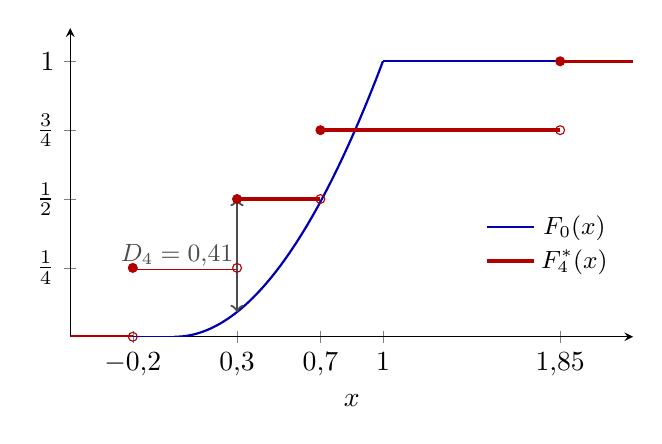
\begin{tikzpicture}
    \begin{axis}[
      width=0.72\textwidth, height=5.5cm,
      xmin=-0.5, xmax=2.2, ymin=0, ymax=1.12,
      axis lines=left, xlabel={$x$}, ylabel={},
      xtick={-0.2, 0.3, 0.7, 1, 1.85},
      xticklabels={$-0{,}2$, $0{,}3$, $0{,}7$, $1$, $1{,}85$},
      ytick={0.25, 0.5, 0.75, 1},
      yticklabels={$\frac14$, $\frac12$, $\frac34$, $1$},
      legend style={draw=none, at={(0.98,0.3)}, anchor=east, font=\small},
    ]
      % F_0(x) = x^2 на [0,1]
      \addplot[thick, blue!70!black, domain=-0.5:0, samples=2] {0};
      \addlegendentry{$F_0(x)$}
      \addplot[thick, blue!70!black, domain=0:1, samples=60, forget plot] {x^2};
      \addplot[thick, blue!70!black, domain=1:2.2, samples=2, forget plot] {1};
      % ступеньки F_4^*
      \addplot[very thick, red!70!black, domain=-0.5:-0.2] {0};
      \addlegendentry{$F_4^*(x)$}
      \addplot[very thick, red!70!black, forget plot] coordinates {(-0.2,0.25) (0.3,0.25)};
      \addplot[very thick, red!70!black, forget plot] coordinates {(0.3,0.5) (0.7,0.5)};
      \addplot[very thick, red!70!black, forget plot] coordinates {(0.7,0.75) (1.85,0.75)};
      \addplot[very thick, red!70!black, forget plot] coordinates {(1.85,1) (2.2,1)};
      \addplot[only marks, mark=*, mark size=1.6pt, red!70!black, forget plot]
        coordinates {(-0.2,0.25) (0.3,0.5) (0.7,0.75) (1.85,1)};
      \addplot[only marks, mark=o, mark size=1.6pt, red!70!black, forget plot]
        coordinates {(-0.2,0) (0.3,0.25) (0.7,0.5) (1.85,0.75)};
      % наибольшее отклонение
      \draw[<->, thick, black!70] (axis cs:0.3,0.09) -- (axis cs:0.3,0.5)
        node[midway, left, font=\small, fill=white, inner sep=1pt] {$D_4 = 0{,}41$};
    \end{axis}
  \end{tikzpicture}
  \caption{Пример~\ref{lec05:ex}: эмпирическая функция $F_4^*$ и гипотетическая
           $F_0(x) = x^2$. Наибольшее отклонение~--- справа от скачка в точке $X_{(2)} = 0{,}3$.}
  \label{lec05:fig:example}
\end{figure}

\subsection{Критерий \texorpdfstring{$\omega^2$}{омега-квадрат} (Крамера--Мизеса--Смирнова)}
\label{lec05:omega}

Гипотезы те же: $H_0 \colon F_\xi = F_0$, $H_1 \colon F_\xi \ne F_0$, $F_0$ непрерывна.
Статистика Колмогорова измеряет \emph{наибольшее} отклонение $F_n^*$ от~$F_0$;
статистика $\omega^2$~--- \emph{среднеквадратичное}:
\[
  \omega_n^2(X_{[n]}) = \int_{-\infty}^{+\infty} \bigl(F_n^*(x) - F_0(x)\bigr)^2 \, dF_0(x).
\]
Интегрирование по $dF_0$ означает: отклонения взвешиваются вероятностью~$F_0$.
Для непрерывной $F_0$ с плотностью~$f_0$ это просто $\int (F_n^* - F_0)^2 f_0(x)\, dx$.

Для вычислений интеграл не нужен: справедливо \emph{точное} равенство
\[
  n\, \omega_n^2(X_{[n]}) = \frac{1}{12n}
    + \sum_{i=1}^{n} \Bigl( F_0\bigl(X_{(i)}\bigr) - \frac{2i-1}{2n} \Bigr)^{2},
\]
где $X_{(1)} < \ldots < X_{(n)}$~--- вариационный ряд. (Проверяется заменой $y = F_0(x)$,
как в лемме~\ref{lec05:lemma}, после чего интеграл $\int_0^1 (G_n^*(y) - y)^2\,dy$
берётся по кускам постоянства~$G_n^*$.) В~\cite[гл.~14, замечание~2.2]{bure}
статистикой критерия называется именно правая часть, $\bar\omega_n^2 = n\,\omega_n^2$.

Свойства~--- те же, что у~$D_n$:
\begin{itemize}
  \item при $H_0$ распределение $\bar\omega_n^2$ зависит только от $n$, а не от $F_0$
        (та же замена $y = F_0(x)$);
  \item для малых $n$ есть таблицы критических точек, для больших~--- предельное
        распределение (при $n \to \infty$). Пусть $\Omega$~--- его функция распределения;
        порог $z_{1-\alpha}$ находят из $\Omega(z_{1-\alpha}) = 1 - \alpha$, и $H_0$
        отвергают при $\bar\omega_n^2 > z_{1-\alpha}$.
\end{itemize}
Подробнее о критерии~--- в учебнике А.\,А.~Боровкова <<Математическая статистика>>
(лектор рекомендовал его для самостоятельного чтения).

\begin{keybox}[Что нужно знать к экзамену]
  \begin{itemize}
    \item Гипотезы $H_0$, $H_1$; требование непрерывности $F_0$; определение $D_n$.
    \item Поведение $D_n$ при $H_0$ ($\toas 0$, по Гливенко--Кантелли) и при $H_1$
          ($\toas \sup_x \abs{F_\xi(x) - F_0(x)} > 0$).
    \item Лемма о том, что распределение $D_n$ не зависит от $F_0$, с доказательством:
          $F_0(\xi) \sim U[0, 1]$, замена $y = F_0(x)$,
          $D_n = \sup_{y \in [0,1]} \abs{G_n^*(y) - y}$.
    \item Теорема Колмогорова: $\P\{\sqrt{n}\, D_n \le z\} \to K(z)$, формула $K(z)$.
    \item Правило: отвергаем $H_0$, если $\sqrt{n}\, D_n > d_{1-\alpha}$
          ($d_{0{,}95} \approx 1{,}36$).
    \item Вычислительная формула для $D_n$ через вариационный ряд и почему хватает
          $2n$ значений.
    \item Статистика $\omega^2$: определение и формула для $n\,\omega_n^2$.
  \end{itemize}
  \emph{Где легко ошибиться:}
  \begin{itemize}
    \item $F_0(\xi)$ распределена \emph{равномерно} на $[0,1]$, а не нормально;
    \item для $D_n \toas 0$ нужна равномерная сходимость (Гливенко--Кантелли), поточечной мало;
    \item с $d_{1-\alpha}$ сравнивают $\sqrt{n}\, D_n$, а не $D_n$;
    \item формула для $\omega^2$~--- точное равенство для $n\,\omega_n^2$, а не
          сходимость; в ней порядковые статистики $X_{(i)}$, а не $X_i$;
    \item $F_0$ должна быть известна полностью: критерий проверяет \emph{простую} гипотезу;
    \item значения $F_0$ берутся по её формуле на всей прямой: например, $F_0(x) = 0$ при $x \le 0$.
  \end{itemize}
\end{keybox}
